\section{Filtros con ventana de Kaiser y Medición en DSP}
Se simularon las siguientes plantillas con la ventana de Kaiser y se corrió el software en el DSP.

\begin{table}[H]
\centering
\begin{tabular}{|c|c|c|c|c|c|c|c|}
\hline
$f_s(Hz)$ & $f_a^-(Hz)$ & $f_p^-(Hz)$ & $f_p^+(Hz)$ & $f_a^+(Hz)$ & $A_p(dB)$ & $A_a(dB)$ & Ventana     \\ \hline
$48k$     & $2k$        & $2.2k$      &   $3k$      &     $3.2k$ &  1         & 40        & Kaiser      \\ \hline
\end{tabular}
\caption{Plantilla del filtro pasabanda.}
\label{tab:3passband}
\end{table}

\begin{table}[H]
\centering
\begin{tabular}{|c|c|c|c|c|c|}
\hline
$f_s(Hz)$ & $f_p(Hz)$ & $f_a(Hz)$ & $A_p(dB)$ & $A_a(dB)$ & Ventana     \\ \hline
$48k$     & $2k$        & $2.2k$  &  1         & 40       & Kaiser      \\ \hline
\end{tabular}
\caption{Plantilla del filtro pasabajos.}
\label{tab:3lowpass}
\end{table}

\begin{table}[H]
\centering
\begin{tabular}{|c|c|c|c|c|c|}
\hline
$f_s(Hz)$ & $f_a(Hz)$ & $f_p(Hz)$ & $A_p(dB)$ & $A_a(dB)$ & Ventana     \\ \hline
$48k$     & $2k$        & $2.2k$  &  1         & 40       & Kaiser      \\ \hline
\end{tabular}
\caption{Plantilla del filtro pasaaltos.}
\label{tab:3hipass}
\end{table}


\subsection{Resultados y análisis de resultados}
\begin{figure}[H]
  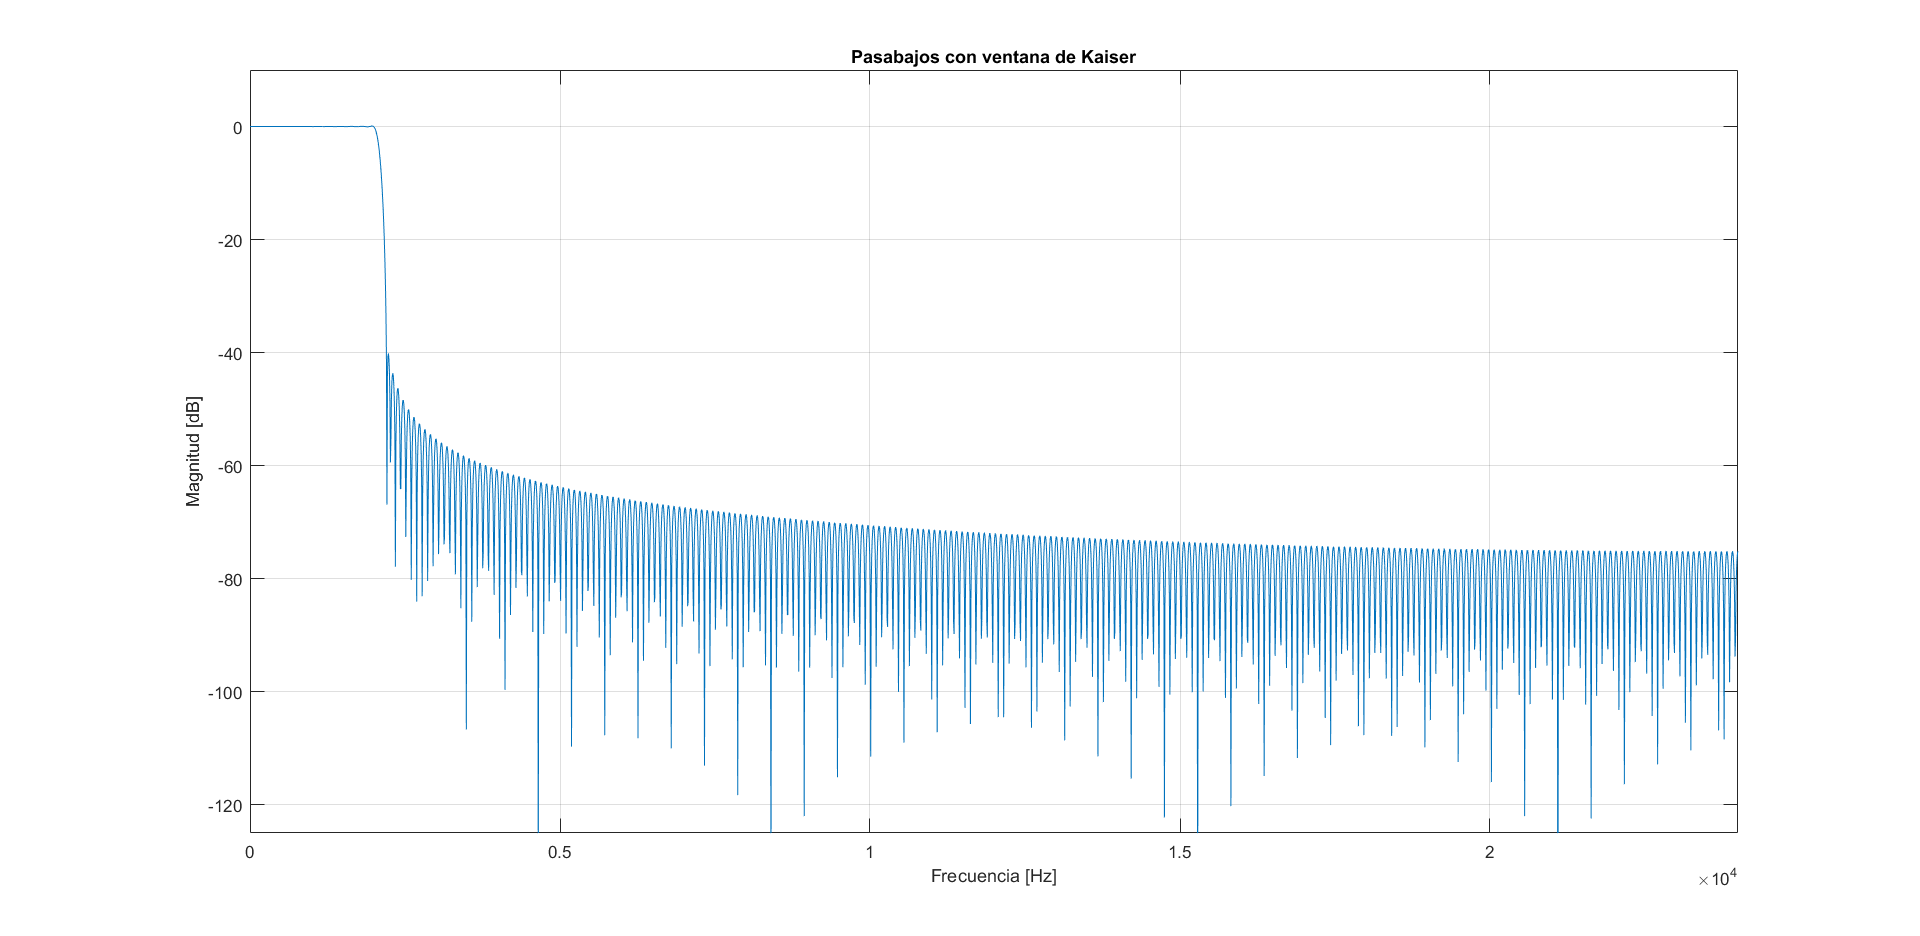
\includegraphics[scale=.35]{./images/3/pasabajoskaisermodulo.png}
  \caption{Respuesta en frecuencia del pasabajos con ventana de Kaiser.}
\end{figure}
\begin{figure}[H]
  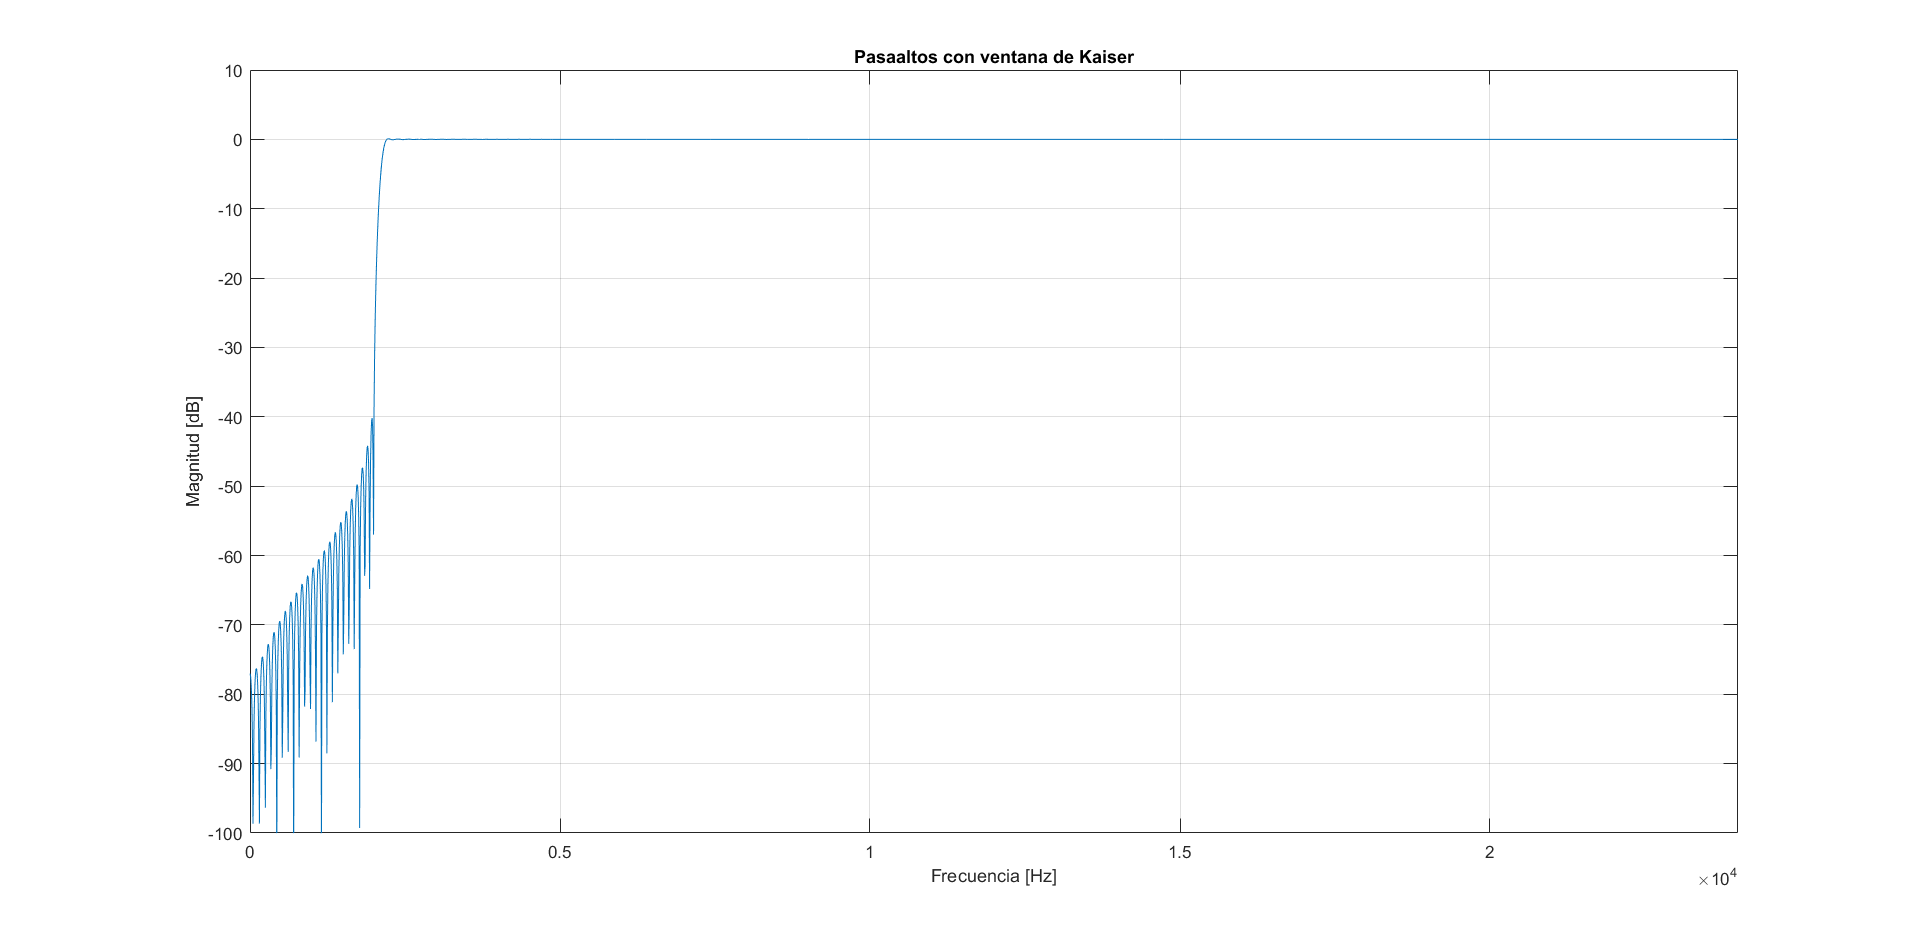
\includegraphics[scale=.35]{./images/3/pasaaltoskaisermodulo.png}
  \caption{Respuesta en frecuencia del pasaaltos con ventana de Kaiser.}
\end{figure}
\subsection{Simulación Pasabanda y Medición en DSP.}
\begin{figure}[H]
  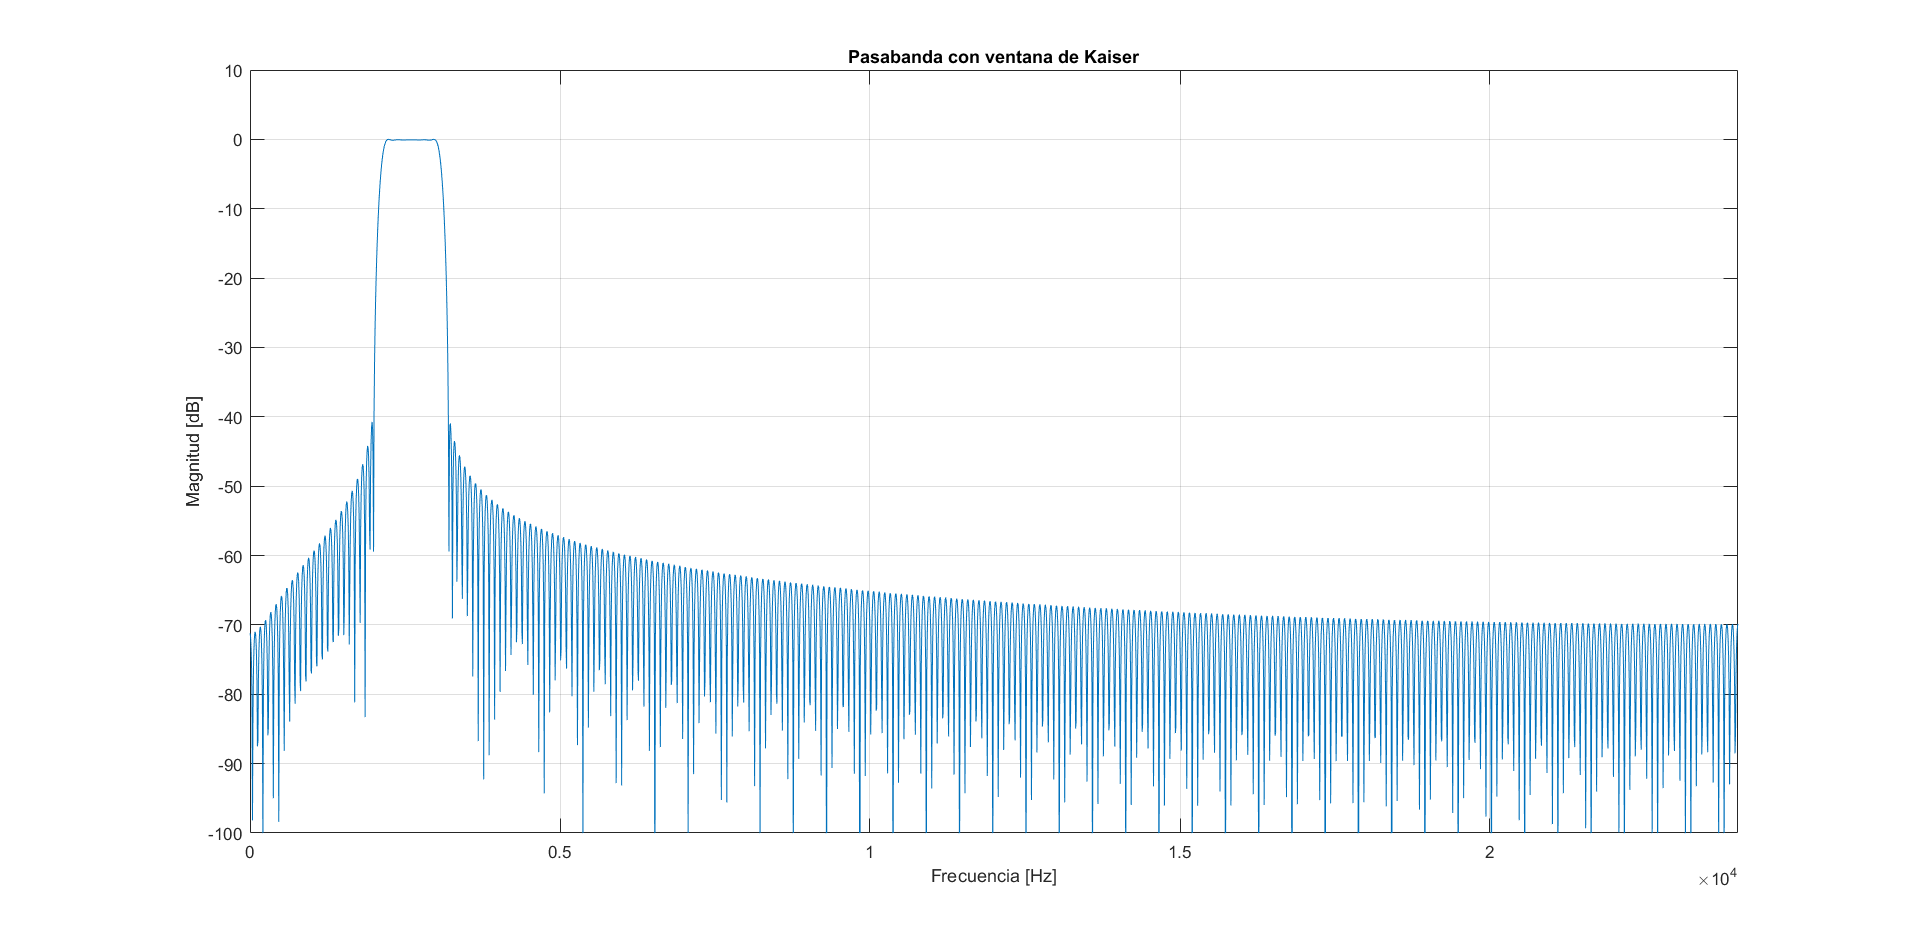
\includegraphics[scale=.35]{./images/3/pasabandakaisermodulo.png}
  \caption{Respuesta en frecuencia del pasabanda con ventana de Kaiser.}
\end{figure}
\begin{figure}[H]
  \centering
  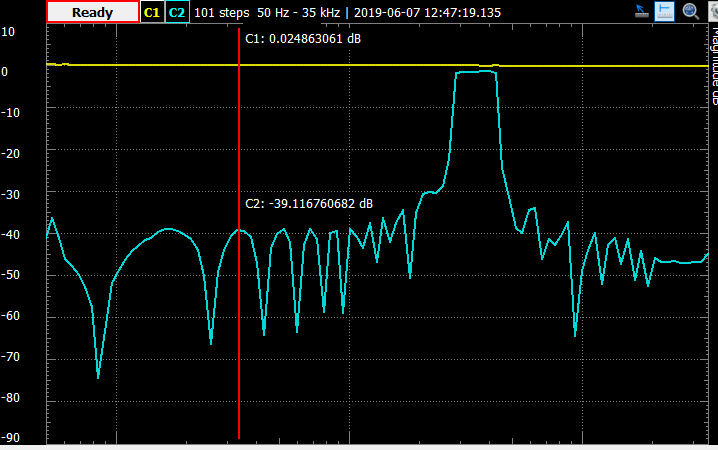
\includegraphics[scale=1]{./images/3/pasabandagrupo2mod.png}
  \caption{Medición del pasabanda en el DSP.}
  \label{fig:dsp}
\end{figure}
Se puede observar que tanto en el caso del pasabajos como del pasaaltos y pasabanda la simulación cumple plantilla. Por otro lado, se simuló en el Procesador de señales DSP56303 y se obtuvieron los resultados mostrados en la figura \refeq{fig:dsp}; con la diferencia mayor siendo la atenuación que se observa en la medición debida al atenuador presente en el procesador.
